\section{Mantle Engine: Methodology}

\subsection{Experimental Setup}

\subsection{Mantle: Dynamic Load Balancing Policies}

%  \item motivation: Mochi load balancer microservice

%  \item background: CephFS implementation

%  \item library architecture, callbacks, environment
We extract Mantle as a library that is linked into a service ({\it e.g.}, file
system, key-value store, application), where administrators program policies
that are embedded into the runtime.  The service needs to be modified to (1)
provide environment of metrics (2) identify where policies are set. At runtime,
Mantle executes the admin's policies for when/where/how much and returns a
decision.

\begin{figure}[t]
  \noindent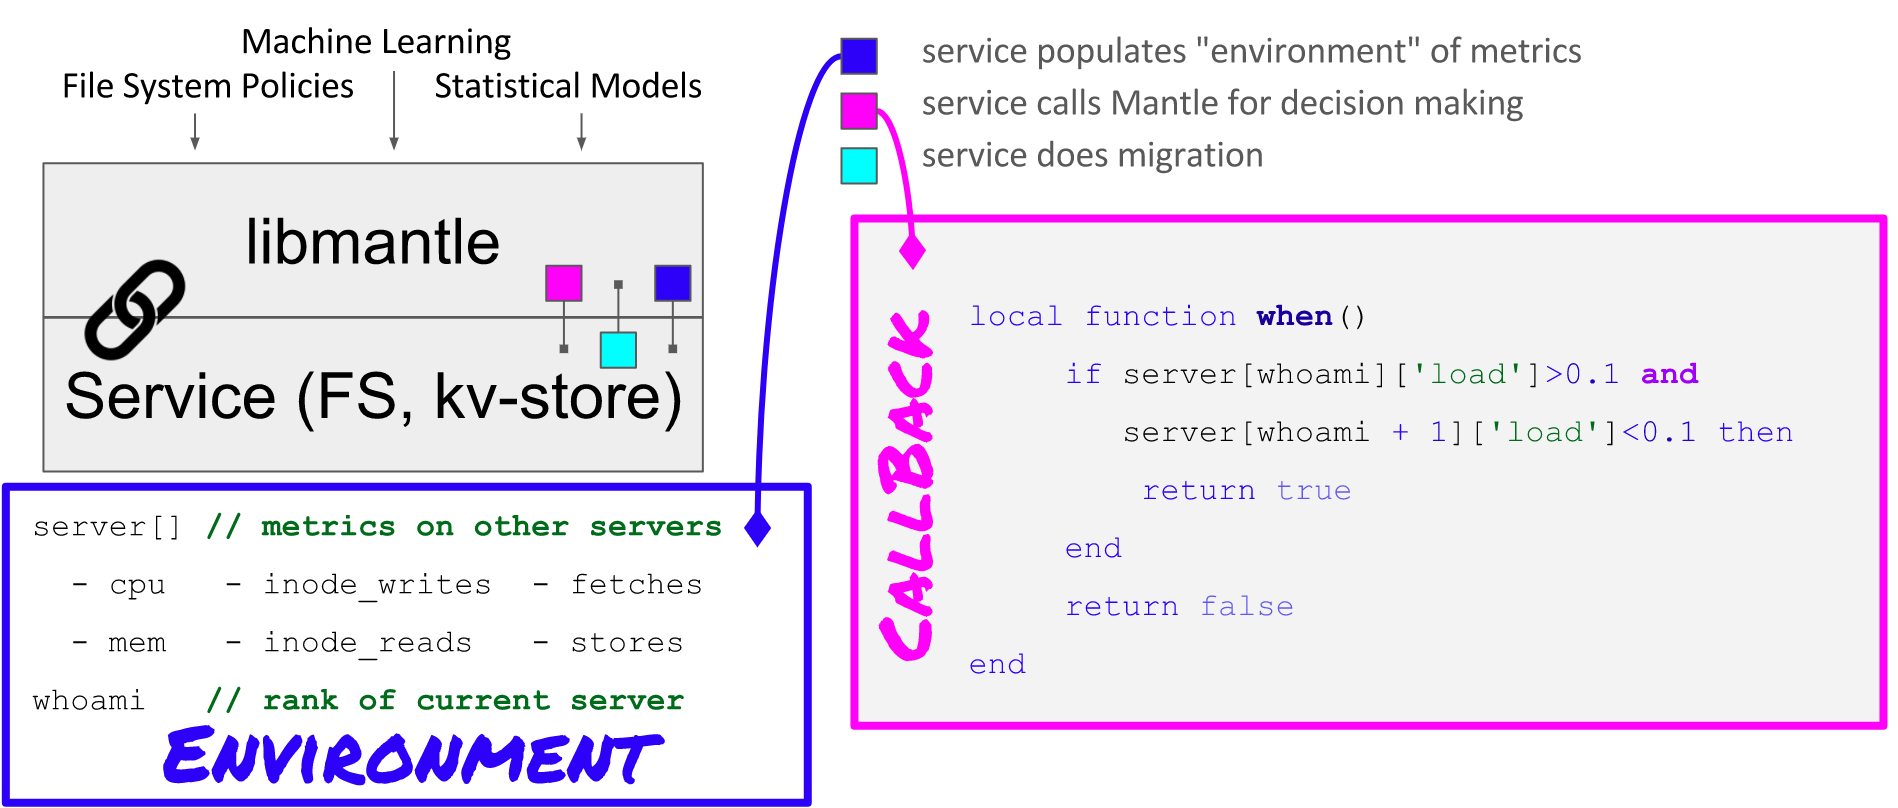
\includegraphics[width=0.5\textwidth]{figures/mantle.png}\\

  \caption{Extracting Mantle as library.\label{fig:mantle}}

\end{figure}

\begin{table}
  \centering
  \begin{tabular}{ r | l | l }
  Metrics     & Data Structure & Description \\\hline
  Cluster     & \{server \(\rightarrow\) \{metric \(\rightarrow\) val\}\}
              & resource util. for servers \\
  Time Series & [(ts, val), ..., (ts, val)]
              & accesses by timestamp (ts) \\
  && \\
              & Service      & Example \\\hline
  Cluster     & File Systems & CPU util., Inode RDs \\
              & ParSplice    & CPU util., Cache Size \\
  Time Series & File Systems & Accesses to directory \\
              & ParSplice    & Accesses to key in DB\\
  \end{tabular}
  \caption{Types of metrics exposed by the service to the policy engine using Mantle.\label{table:metrics}}
\end{table}

%of timestamp (ts), value pairs representing accesses over time types of
%metrics: key value pairs
Services expose two types of metrics with Mantle: cluster metrics for
describing resource utilization and time series metrics for describing accesses
over time. Table~\ref{table:metrics} shows how these metrics are accessed from
the policies written by administrators. Cluster metrics are read from a
dictionary indexed by server and metric name, where server is a node identifier
({e.g.}, MPI Rank, metadata server name), metric is a resource name and val is
the current reading for that metric.  Examples of \texttt{(metric, value)}
pairs are CPU or memory pressure, as shown in Figure~\ref{fig:mantle}.  For
time series metrics, the service passes a pointer to an array of
\texttt{(timestamp, value)} pairs. We use a pointer so we can pass a large
number of values, like accesses over time to a database or directory in the
file system namespace, but this limits the time series metrics to only include
values from the {\it current } node.

% policies themselves
Administrators write policies as callbacks that use the metrics from above.
Figure~\ref{fig:mantle} shows an example policy for the ``when()" callback, where the
current server (\texttt{whoami}) migrates load if it is has load
(\texttt{>0.1}) and if its neighbor server (\texttt{whoami + 1}) does not have
load (\texttt{<0.1}). 

\subsection{Integrating Mantle into ParSplice}

\begin{itemize}
  \item providing environment of metrics
  \item identifying where policies are made
\end{itemize}
